% The Slide Definitions
%document
\documentclass[10pt]{beamer}
%theme
\usetheme{metropolis}
% packages
\usepackage{color}
\usepackage{listings}
\usepackage[ngerman]{babel}
\usepackage[utf8]{inputenc}
\usepackage{multicol}


% color definitions
\definecolor{mygreen}{rgb}{0,0.6,0}
\definecolor{mygray}{rgb}{0.5,0.5,0.5}
\definecolor{mymauve}{rgb}{0.58,0,0.82}

\lstset{
    backgroundcolor=\color{white},
    % choose the background color;
    % you must add \usepackage{color} or \usepackage{xcolor}
    basicstyle=\footnotesize\ttfamily,
    % the size of the fonts that are used for the code
    breakatwhitespace=false,
    % sets if automatic breaks should only happen at whitespace
    breaklines=true,                 % sets automatic line breaking
    captionpos=b,                    % sets the caption-position to bottom
    commentstyle=\color{mygreen},    % comment style
    % deletekeywords={...},
    % if you want to delete keywords from the given language
    extendedchars=true,
    % lets you use non-ASCII characters;
    % for 8-bits encodings only, does not work with UTF-8
    frame=single,                    % adds a frame around the code
    keepspaces=true,
    % keeps spaces in text,
    % useful for keeping indentation of code
    % (possibly needs columns=flexible)
    keywordstyle=\color{blue},       % keyword style
    % morekeywords={*,...},
    % if you want to add more keywords to the set
    numbers=left,
    % where to put the line-numbers; possible values are (none, left, right)
    numbersep=5pt,
    % how far the line-numbers are from the code
    numberstyle=\tiny\color{mygray},
    % the style that is used for the line-numbers
    rulecolor=\color{black},
    % if not set, the frame-color may be changed on line-breaks
    % within not-black text (e.g. comments (green here))
    stepnumber=1,
    % the step between two line-numbers.
    % If it's 1, each line will be numbered
    stringstyle=\color{mymauve},     % string literal style
    tabsize=4,                       % sets default tabsize to 4 spaces
    % show the filename of files included with \lstinputlisting;
    % also try caption instead of title
    language = Python,
	showspaces = false,
	showtabs = false,
	showstringspaces = false,
	escapechar = ,
}

\def\ContinueLineNumber{\lstset{firstnumber=last}}
\def\StartLineAt#1{\lstset{firstnumber=#1}}
\let\numberLineAt\StartLineAt



\newcommand{\codeline}[1]{
	\alert{\texttt{#1}}
}


% Author and Course information
% This Document contains the information about this course.

% Authors of the slides
\author{Philipp Hanisch, Valentin Roland}

% Name of the Course
\institute{Python-Grundlagen}

% Fancy Logo 
\titlegraphic{\hfill
\includegraphics[height=1.25cm]{fsr_logo_cropped}}



% Custom Bindings
% \newcommand{\codeline}[1]{
%	\alert{\texttt{#1}}
%}


% Presentation title
\title{Objektorientierung (II) und Modularisierung}
\date{\today}


\begin{document}

\maketitle

\begin{frame}{Gliederung}
    \setbeamertemplate{section in toc}[sections numbered]
    \tableofcontents
\end{frame}

% ---- Rückblick ----
\section{Rückblick: Objektorientierung}

\begin{frame}{Objekte und Klassen}
    \begin{itemize}
	\item \textbf{Objekte} haben Eigenschaften (\textbf{Attribute}) und Verhalten (\textbf{Methoden})
	\item Objekte als \textbf{Instanzen} (Ausprägungen) einer \textbf{Klasse} 
	\item Klassen als \glqq Schablone\grqq{} oder \glqq Bauplan\grqq{} für Objekte
	\item Objekte einer Klasse haben gleiche Attribute, die einen unterschiedlichen Wert haben können
    \end{itemize}
    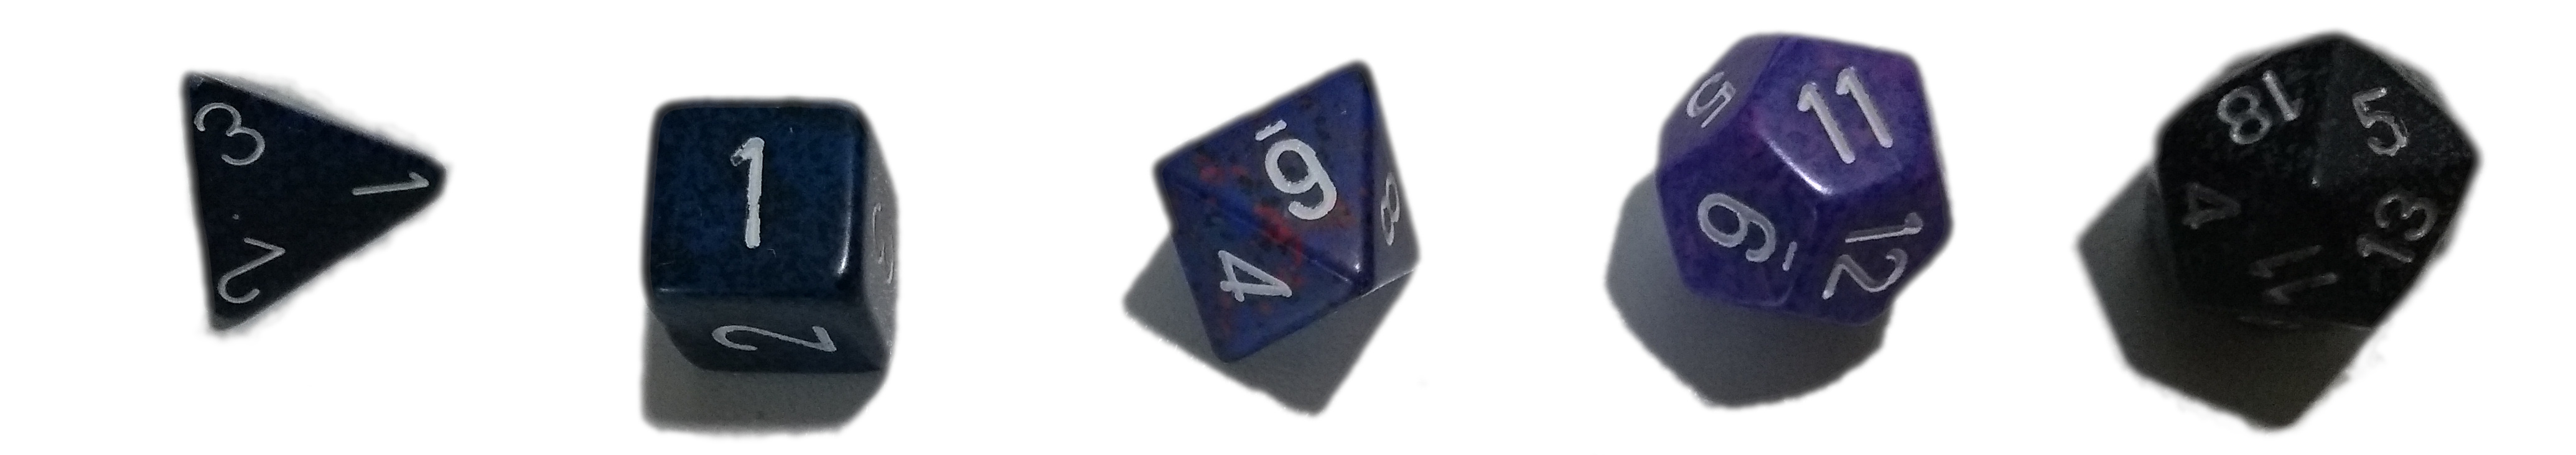
\includegraphics[width=\textwidth]{dice.jpg}
\end{frame}

  %  \begin{center}
  %      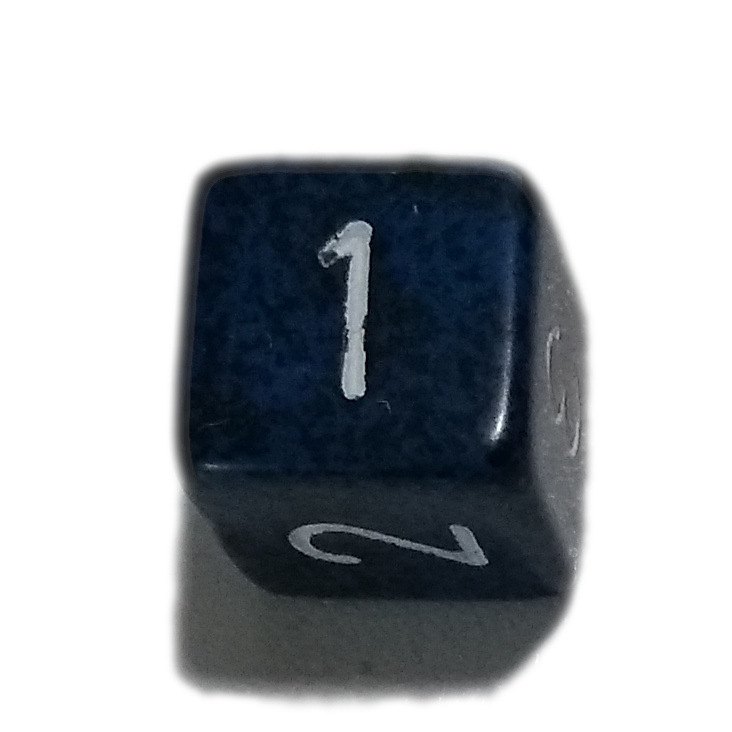
\includegraphics[width=0.5\textwidth]{d6.jpg}
  %  \end{center}
  %  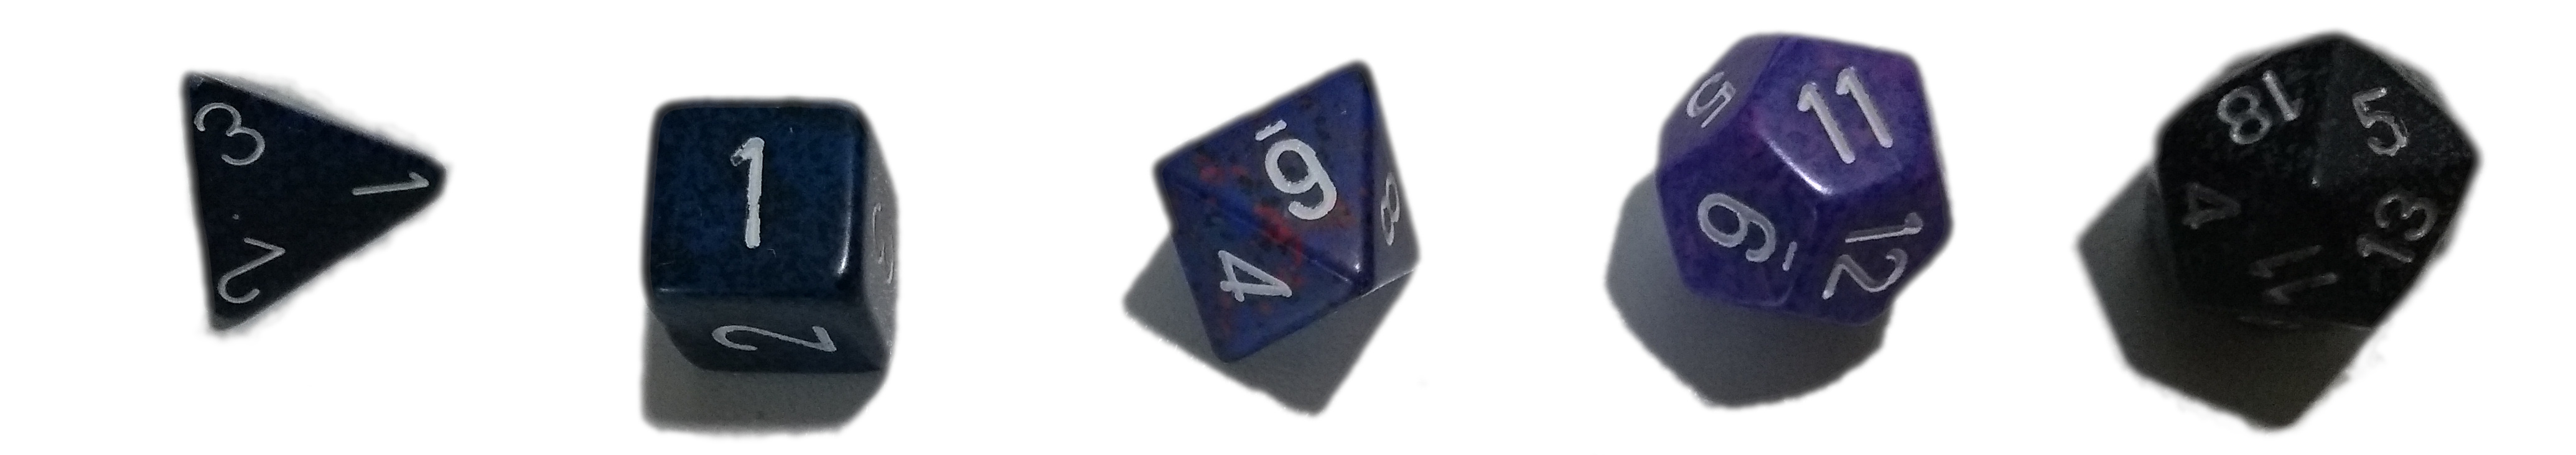
\includegraphics[width=\textwidth]{dice.jpg}

\begin{frame}{Aufgabenstellung}
    \begin{enumerate}
        \item Implementiere die Würfelklasse und erzeuge einige Würfel und würfel!
        \item Schreibe eine Klasse \glqq Spieler\grqq!
        \item Erweitere dein Würfelspiel, sodass zwei Spielerobjekte gegeneinander spielen.
        \item Auch abstrakte Konzepte können als Klasse modelliert werden. Wie könnte man ein Würfelspiel mit mehreren Runden als Klasse darstellen?
    \end{enumerate}
\end{frame}


\begin{frame}[fragile]{Lösung}
    \begin{lstlisting}
from random import randint

class Wuerfel:
    def __init__(self, seiten):
        self.seiten = seiten

    def wuerfeln(self):
        return randint(1, self.seiten)


d6 = Wuerfel(6)
d20 = Wuerfel(20)

print("Du hast eine {} gewürfelt!".format(d20.wuerfeln()))

d20.seiten = 12
print(d20.seiten)
    \end{lstlisting}
\end{frame}


\begin{frame}[fragile]{Lösung}
	\begin{lstlisting}
class Spieler:
    def __init__(self, name, wuerfel):
        self.name = name
        self.wuerfel = wuerfel

    def wuerfel_wecheln(self, wuerfel):
        self.wuerfel = wuerfel

    def wuerfeln(self):
        return self.wuerfel.wuerfeln()


d20 = Wuerfel(20)
spieler = Spieler("Laucian", d20)

wurf = spieler.wuerfeln()
print("{} hat eine {} gewürfelt!".format(spieler.name, wurf))
spieler.wuerfel = Wuerfel(12)
	\end{lstlisting}
\end{frame}

% ----------------------- Modularisierung in Python -----------------------

\section{Modularisierung}

\begin{frame}{Motivation}
	\begin{itemize}
		\item Struktur und Übersichtlichkeit 
		\item Wiederverwendung (z.B. mathematische Funktionen)
		\item Nutzung von Bibliotheken (z.B. random)
		\item (einheitliche) Definition von Konstanten, Klassen, etc.
	\end{itemize}
\end{frame}


\begin{frame}[fragile]{Module einbinden}
	\begin{lstlisting}
from random import randint
print(randint(1, 10))

from wuerfel import *
d20 = Wuerfel(20)
print(d20.wuerfeln())

import spieler
spieler = spieler.Spieler("Arndt", d20)
print(spieler.name)
	\end{lstlisting}
\end{frame}


\begin{frame}[fragile]{Boilerplate}
	\begin{lstlisting}
class Wuerfel:
    def __init__(self, seiten):
        self.seiten = seiten
	
    # weitere Methoden

if __name__ == '__main__': # Boilerplate
    # Code wird beim Importieren nicht ausgeführt
    d20 = Wuerfel(20)
    print(d20.wuerfeln())
	\end{lstlisting}

	\texttt{\_\_name\_\_} enthält den Namen des Scriptes beim Importieren
	oder \texttt{'\_\_main\_\_'}, wenn das Script direkt ausgeführt wird.

\end{frame}


% --------------------- Aufgaben -------------------------

\section{Aufgaben}

\begin{frame}{Aufgaben}
	\begin{enumerate}
		\item Erweitere die Spielerklasse, sodass ein Spieler mehrere Würfel besitzen kann. Wenn er würfelt, so soll er mit allen Würfeln nacheinander würfeln und eine Ergebnisliste zurückbekommen.
		\item Modelliert das Würfelspiel als eigene Klasse.
			\begin{enumerate}
				\item Das Spiel sollte (min.) zwei Spieler umfassen, die in Runden gegeneinander spielen.
				\item Wie ist der jeweilige Zwischenstand?
				\item Wie sieht eine Runde aus? Würfeln die Spieler mit einem Würfel? Mit mehreren? Gewinnt die höchste Summe? Oder der höchste Wert?
				\item Strukturiert euren Code so, dass die Änderung, was eine Runde ist, möglichst wenig Änderungen im Code bedeutet.
			\end{enumerate}
	\end{enumerate}
\end{frame}

\begin{frame}{Aufgaben}
	\begin{enumerate}
		\setcounter{enumi}{3}
		\item Modifiziert eure Spieler, um folgende Sachverhalte zu modellieren.
			\begin{enumerate}
				\item Wenn ein Spieler mit \textit{Vorteil} würfelt, so würfelt er zweimal und der höhere Wert zählt. Gleichermaßen kann er einen \textit{Nachteil} haben (niedrigerer Wert). Vorteil und Nachteil gleichzeitig führen zu einem normalen Würfelwurf.
				\item Ein Spieler verfügt über einen \textit{Bonus}, der zu jedem Wurf dazu addiert wird.
				\item Ein Spieler kann seinen Bonus erhöhen, Vorteil oder Nachteil erhalten oder verlieren.
			\end{enumerate}
		\item Wie viel Bonus braucht ein Spieler, damit das Spiel ausgeglichen ist, wenn sein Gegner Vorteil auf jeden Wurf hat? Wie viel, wenn unser Spieler gleichzeitig Nachteil hat?
		\item Überlegt euch weitere (interessante) Würfelspiele.
	\end{enumerate}
\end{frame}

\end{document}
